% Options for packages loaded elsewhere
% Options for packages loaded elsewhere
\PassOptionsToPackage{unicode}{hyperref}
\PassOptionsToPackage{hyphens}{url}
\PassOptionsToPackage{dvipsnames,svgnames,x11names}{xcolor}
%
\documentclass[
  ngerman,
  number,
  preprint,
  3p,
  twocolumn]{elsarticle}
\usepackage{xcolor}
\usepackage{amsmath,amssymb}
\setcounter{secnumdepth}{5}
\usepackage{iftex}
\ifPDFTeX
  \usepackage[T1]{fontenc}
  \usepackage[utf8]{inputenc}
  \usepackage{textcomp} % provide euro and other symbols
\else % if luatex or xetex
  \usepackage{unicode-math} % this also loads fontspec
  \defaultfontfeatures{Scale=MatchLowercase}
  \defaultfontfeatures[\rmfamily]{Ligatures=TeX,Scale=1}
\fi
\usepackage{lmodern}
\ifPDFTeX\else
  % xetex/luatex font selection
\fi
% Use upquote if available, for straight quotes in verbatim environments
\IfFileExists{upquote.sty}{\usepackage{upquote}}{}
\IfFileExists{microtype.sty}{% use microtype if available
  \usepackage[]{microtype}
  \UseMicrotypeSet[protrusion]{basicmath} % disable protrusion for tt fonts
}{}
\makeatletter
\@ifundefined{KOMAClassName}{% if non-KOMA class
  \IfFileExists{parskip.sty}{%
    \usepackage{parskip}
  }{% else
    \setlength{\parindent}{0pt}
    \setlength{\parskip}{6pt plus 2pt minus 1pt}}
}{% if KOMA class
  \KOMAoptions{parskip=half}}
\makeatother
% Make \paragraph and \subparagraph free-standing
\makeatletter
\ifx\paragraph\undefined\else
  \let\oldparagraph\paragraph
  \renewcommand{\paragraph}{
    \@ifstar
      \xxxParagraphStar
      \xxxParagraphNoStar
  }
  \newcommand{\xxxParagraphStar}[1]{\oldparagraph*{#1}\mbox{}}
  \newcommand{\xxxParagraphNoStar}[1]{\oldparagraph{#1}\mbox{}}
\fi
\ifx\subparagraph\undefined\else
  \let\oldsubparagraph\subparagraph
  \renewcommand{\subparagraph}{
    \@ifstar
      \xxxSubParagraphStar
      \xxxSubParagraphNoStar
  }
  \newcommand{\xxxSubParagraphStar}[1]{\oldsubparagraph*{#1}\mbox{}}
  \newcommand{\xxxSubParagraphNoStar}[1]{\oldsubparagraph{#1}\mbox{}}
\fi
\makeatother


\usepackage{longtable,booktabs,array}
\usepackage{calc} % for calculating minipage widths
% Correct order of tables after \paragraph or \subparagraph
\usepackage{etoolbox}
\makeatletter
\patchcmd\longtable{\par}{\if@noskipsec\mbox{}\fi\par}{}{}
\makeatother
% Allow footnotes in longtable head/foot
\IfFileExists{footnotehyper.sty}{\usepackage{footnotehyper}}{\usepackage{footnote}}
\makesavenoteenv{longtable}
\usepackage{graphicx}
\makeatletter
\newsavebox\pandoc@box
\newcommand*\pandocbounded[1]{% scales image to fit in text height/width
  \sbox\pandoc@box{#1}%
  \Gscale@div\@tempa{\textheight}{\dimexpr\ht\pandoc@box+\dp\pandoc@box\relax}%
  \Gscale@div\@tempb{\linewidth}{\wd\pandoc@box}%
  \ifdim\@tempb\p@<\@tempa\p@\let\@tempa\@tempb\fi% select the smaller of both
  \ifdim\@tempa\p@<\p@\scalebox{\@tempa}{\usebox\pandoc@box}%
  \else\usebox{\pandoc@box}%
  \fi%
}
% Set default figure placement to htbp
\def\fps@figure{htbp}
\makeatother



\ifLuaTeX
\usepackage[bidi=basic]{babel}
\else
\usepackage[bidi=default]{babel}
\fi
% get rid of language-specific shorthands (see #6817):
\let\LanguageShortHands\languageshorthands
\def\languageshorthands#1{}
\ifLuaTeX
  \usepackage[german]{selnolig} % disable illegal ligatures
\fi


\setlength{\emergencystretch}{3em} % prevent overfull lines

\providecommand{\tightlist}{%
  \setlength{\itemsep}{0pt}\setlength{\parskip}{0pt}}



 
\usepackage[]{natbib}
\bibliographystyle{plainnat}


\makeatletter
\@ifpackageloaded{caption}{}{\usepackage{caption}}
\AtBeginDocument{%
\ifdefined\contentsname
  \renewcommand*\contentsname{Inhaltsverzeichnis}
\else
  \newcommand\contentsname{Inhaltsverzeichnis}
\fi
\ifdefined\listfigurename
  \renewcommand*\listfigurename{Abbildungsverzeichnis}
\else
  \newcommand\listfigurename{Abbildungsverzeichnis}
\fi
\ifdefined\listtablename
  \renewcommand*\listtablename{Tabellenverzeichnis}
\else
  \newcommand\listtablename{Tabellenverzeichnis}
\fi
\ifdefined\figurename
  \renewcommand*\figurename{Abbildung}
\else
  \newcommand\figurename{Abbildung}
\fi
\ifdefined\tablename
  \renewcommand*\tablename{Tabelle}
\else
  \newcommand\tablename{Tabelle}
\fi
}
\@ifpackageloaded{float}{}{\usepackage{float}}
\floatstyle{ruled}
\@ifundefined{c@chapter}{\newfloat{codelisting}{h}{lop}}{\newfloat{codelisting}{h}{lop}[chapter]}
\floatname{codelisting}{Listing}
\newcommand*\listoflistings{\listof{codelisting}{Listingverzeichnis}}
\makeatother
\makeatletter
\makeatother
\makeatletter
\@ifpackageloaded{caption}{}{\usepackage{caption}}
\@ifpackageloaded{subcaption}{}{\usepackage{subcaption}}
\makeatother
\usepackage{float}
\makeatletter
\let\oldlt\longtable
\let\endoldlt\endlongtable
\def\longtable{\@ifnextchar[\longtable@i \longtable@ii}
\def\longtable@i[#1]{\begin{figure}[H]
\onecolumn
\begin{minipage}{0.5\textwidth}
\oldlt[#1]
}
\def\longtable@ii{\begin{figure}[H]
\onecolumn
\begin{minipage}{0.5\textwidth}
\oldlt
}
\def\endlongtable{\endoldlt
\end{minipage}
\twocolumn
\end{figure}}
\makeatother
\usepackage{bookmark}
\IfFileExists{xurl.sty}{\usepackage{xurl}}{} % add URL line breaks if available
\urlstyle{same}
\hypersetup{
  pdftitle={Update Facharztmangel im ÖGD},
  pdfauthor={Jakob Schumacher; Peter Tinnemann},
  pdflang={de},
  pdfkeywords={Facharzt},
  colorlinks=true,
  linkcolor={blue},
  filecolor={Maroon},
  citecolor={Blue},
  urlcolor={Blue},
  pdfcreator={LaTeX via pandoc}}


\setlength{\parindent}{6pt}
\begin{document}

\begin{frontmatter}
\title{Update Facharztmangel im ÖGD \\\large{Haben die Entwicklungen
rund um die Coronapandemie die Anzahl an Fachärzten für öffentliches
Gesundheitswesen erhöht?} }
\author[1]{Jakob Schumacher%
%
}
 \ead{schumacherj@rki.de} 
\author[2]{Peter Tinnemann%
%
}


\affiliation[1]{organization={Robert Koch-Institut},,postcodesep={}}
\affiliation[2]{organization={Gesundheitsamt Frankfurt},,postcodesep={}}

\cortext[cor1]{Corresponding author}


        





\begin{keyword}
    Facharzt \sep 
    Facharzt
\end{keyword}
\end{frontmatter}
    

\section{Einleitung}\label{einleitung}

Die Studie von Tinnemann et al.~(2021) analysiert die Entwicklung des
Anzahl an Fachärztinnen und Fachärzten für Öffentliches Gesundheitswesen
(ÖGW) in Deutschland. Dabei wurde festgestellt, dass die Gesamtzahl der
Fachärzte in Deutschland um 52 \% gestiegen ist. Die Anzahl der
Fachärzte für ÖGW ist um fast 30 \% zurückgegangen. Die Untersuchung
zeigt auch regionale Unterschiede. Die Studie zeigte auch, die
Fachärztinnen und Fachärzte für ÖGW im Zeitraum im Schnitt älter
geworden sind. Die Autoren weisen darauf hin, dass diese Entwicklungen
die fachärztliche Bearbeitung hoheitlicher Aufgaben und die Versorgung
vulnerabler Bevölkerungsgruppen gefährden.

Die COVID-19-Pandemie führte zu einer Belastung der Gesundheitsämter. Um
die Anforderungen an Infektionsschutz, Kontaktnachverfolgung, Testungen
und Impfungen zu bewältigen, wurde das Personal kurzfristig aufgestockt.
So wurden deutschlandweit etwa 5.900 zusätzliche Beschäftigte
eingestellt. Dieses erfolgte zum Beispiel durch Umschichtungen aus
anderen Verwaltungsbereichen. Mit dem „Pakt für den Öffentlichen
Gesundheitsdienst`` wurden 1.775 unbefristete Stellen geschaffen. Diese
wurden finanziert durch Bundesmittel und hatten das Ziel den
Öffentlichen Gesundheitsdienst (ÖGD) langfristig zu stärken. Wäre dieser
Maßnahmen wurden viele reguläre Aufgaben zurückgestellt, da ein Großteil
des vorhandenen Personals für pandemiebedingte Tätigkeiten eingesetzt
wurde. Gleichzeitig zeigten sich strukturelle Schwächen, wie der Mangel
an Fachärzten für Öffentliches Gesundheitswesen und die Abhängigkeit von
kurzfristigen Lösungen wie der Rekrutierung von Studierenden oder
Rentnern. Diese Entwicklungen verdeutlichen die Notwendigkeit einer
nachhaltigen Personalplanung und -ausstattung im ÖGD, um zukünftige
Krisen besser bewältigen zu können.

Am 12. Dezember 2023 wurde ein Zwischenbericht zum „Pakt für den
Öffentlichen Gesundheitsdienst`` veröffentlicht, der die Fortschritte
und Herausforderungen bei der Personalentwicklung im ÖGD darlegt. Im
Rahmen des Paktes wurden bis Ende 2021 bundesweit 2.290 neue
Vollzeitäquivalente (VZÄ) geschaffen, von denen 1.775 Stellen aus
Paktmitteln finanziert wurden. Etwa 92 \% dieser Stellen entfielen auf
die unteren Gesundheitsbehörden und örtlichen Gesundheitsämter, während
der Rest auf Landesstellen und oberste Landesbehörden verteilt wurde.
Bis Ende 2022 stieg die Zahl der aus Paktmitteln finanzierten Stellen
auf insgesamt rund 3.930 VZÄ, wobei der Schwerpunkt weiterhin auf den
unteren Gesundheitsbehörden lag. Die Besetzung der Stellen erfolgte
gestaffelt über mehrere Jahre, um Kapazitätsprobleme bei der Ausbildung
und Rekrutierung qualifizierten Fachpersonals zu berücksichtigen. Neben
ärztlichem Personal wurden auch Stellen für weiteres Fachpersonal wie
Sozialarbeiter, Hygienekontrolleurinnen und Verwaltungskräfte
geschaffen. Der Bericht zeigt, dass die Umsetzung des Paktes eine
zentrale Rolle bei der Stärkung des ÖGD spielt und die strukturelle
Modernisierung des öffentlichen Gesundheitswesens unterstützt.

Die Studie analysiert die Verteilung und den Bedarf an
Public-Health-Professionals in deutschen Gesundheitsämtern. Mittels
einer Online-Befragung von 376 Amtsleitungen (Teilnahmerate: 40,4 \%)
wurde festgestellt, dass durchschnittlich 2,6
Public-Health-Professionals pro Gesundheitsamt beschäftigt sind, wobei
28,3 \% der Ämter keine solchen Fachkräfte haben. 78,3 \% der Befragten
äußerten Bedarf an zusätzlichem Personal, insbesondere mit
Public-Health-Qualifikationen. Die Ergebnisse zeigen eine heterogene
Verteilung und verdeutlichen die Notwendigkeit einer stärkeren
Zusammenarbeit zwischen akademischer Public Health und dem Öffentlichen
Gesundheitsdienst (ÖGD), um multiprofessionelle Strukturen auszubauen
und Karrierechancen für Public-Health-Absolventen zu verbessern.

\subsection{Fragestellung}\label{fragestellung}

Haben die Entwicklungen rund um die Coronapandemie die Anzahl an
Fachärzten für öffentliches Gesundheitswesen erhöht?

\section{Methoden}\label{methoden}

Die Ärztestatistik basiert auf den Heilberufsgesetzen der Bundesländer,
die Ärztekammer-Mitgliedschaft vorschreiben. Die Kammern führen
Verzeichnisse ihrer Mitglieder und erstellen jährlich Auswertungen, die
an die Bundesärztekammer (BÄK) übermittelt werden. Die BÄK fasst diese
Daten zusammen und erstellt eine bundesweite Statistik, die
Informationen zu Ärzten mit Gebiets- und Facharztbezeichnungen enthält.

\textsubscript{Quelle:
\href{https://jakobschumacher.github.io/Update-Facharztmangel-im-oeffentlichen-Gesundheitsdienst/index.qmd.html}{Artikel-Notizbuch}}

\textsubscript{Quelle:
\href{https://jakobschumacher.github.io/Update-Facharztmangel-im-oeffentlichen-Gesundheitsdienst/index.qmd.html}{Artikel-Notizbuch}}

\subsection{Datenquelle}\label{datenquelle}

Die Daten stammen von den Ärztekammern. Sie werden bereitgestellt auf
\url{http://www.gbe-bund.de} unter dem Tabellennamen:
\href{http://www.gbe-bund.de/gbe10/express.prc_expr?p_aid=30416728&p_uid=gast&p_sprachkz=D&p_var=0&nummer=656&p_indsp=&p_ityp=H&p_hlpnr=3&p_lfd_nr=1&p_sprache=D&p_news=&p_janein=J}{``Ärztinnen
und Ärzte mit Gebiets- und Facharztbezeichnung, BÄK''}

Beschreibung der Methodik der Statistik der Mitglieder der (Landes-)
Ärztekammern (Ärztestatistik) von gbe-bund.de

\begin{itemize}
\tightlist
\item
  \emph{In den Heilberufsgesetzen der Bundesländer ist festgelegt, dass
  alle Ärzte, die in einem bestimmten Bundesland tätig sind oder, falls
  sie ihren Beruf nicht ausüben, ihren gewöhnlichen Aufenthalt haben,
  Mitglied der jeweiligen (Landes-) Ärztekammer sein müssen. Die Kammern
  haben über ihre Mitglieder ein Verzeichnis zu führen, in das bestimmte
  Angaben einzutragen sind. Auf der Basis dieser Mitgliederverzeichnisse
  erstellen die (Landes-) Ärztekammern zum 31. Dezember jeden Jahres
  Auswertungen zu ausgewählten Aspekten der Berufspolitik, die sie an
  die Bundesärztekammer weiterleiten. Die Bundesärztekammer (BÄK),
  Arbeitsgemeinschaft der deutschen Ärztekammern, ist die
  Berufsvertretung aller deutschen Ärzte auf Bundesebene. Die
  Bundesärztekammer fasst diese Meldungen zum Bundesergebnis zusammen
  und erstellt somit die Ärztestatistik.}
\end{itemize}

Klick-Beschreibung der Auswahl für den Datensatz: taetigkeit\_facharzt
1. Auswahl der Tabelle ``Ärztinnen und Ärzte mit Gebiets- und
Facharztbezeichnung, BÄK'' auf GBE-Bund.de 1. Nach klick auf
``Werteauswahl einblenden'' und ``Jahr'' alle Jahre anklicken oder
``Markierung für alle Merkmalsausprägungen'' auswählen, dann ``Werte
übernehmen'' anklicken 1. Unter ``Merkmal in Zeilen oder Spalten
ändern'' die folgenden Einstellungen tätigen:
``Gebiets-/Facharztbezeichnung'' in Zeile; ``Tätigkeitsbereich'' in
Zeile; ``Jahr'' in Spalte. Dann auf ``Übernehmen'' klicken 1.
Abspeichern der Datei als csv mit dem Namen:
\emph{taetigkeit\_facharzt.csv} und im Ordner ``data'' abspeichern

Klick-Beschreibung der Auswahl für den Datensatz: region\_facharzt 1.
Auswahl der Tabelle ``Ärztinnen und Ärzte mit Gebiets- und
Facharztbezeichnung, BÄK'' auf GBE-Bund.de 1. Nach Klick auf
``Werteauswahl einblenden'' und ``Jahr'' alle Jahre anklicken oder
``Markierung für alle Merkmalsausprägungen'' auswählen, dann ``Werte
übernehmen'' anklicken 1. Nach Klick auf ``Werteauswahl einblenden'' und
``Darstellung'' alle Punkte auswählen, dann ``Ausgewählte
Merkmalsausprägung (ohne übergeordnete)'' auswählen, dann ``Werte
übernehmen'' anklicken 1. Unter ``Merkmal in Zeilen oder Spalten
ändern'' die folgenden Einstellungen tätigen:
``Gebiets-/Facharztbezeichnung'' in Zeile; ``Region'' in Zeile; ``Jahr''
in Spalte. ``Darstellung'' auf in Zeile; dann auf ``Übernehmen'' klicken
1. Unter ``Auswahl einer neuen Merkmalsausprägung'' in der Zeile
Tätigkeitsbereich den Punkt: ``Mit ärztlicher Tätigkeit'' auswählen dann
``Blattmerkmale aktualisieren'' klicken. 1. Abspeichern der Datei als
csv mit dem Namen: \emph{region\_facharzt.csv} und im Ordner ``data''
abspeichern

Klick-Beschreibung der Auswahl für den Datensatz: geschlecht\_alter 1.
Auswahl der Tabelle ``Ärztinnen und Ärzte mit Gebiets- und
Facharztbezeichnung, BÄK'' auf GBE-Bund.de 1. Nach Klick auf
``Werteauswahl einblenden'' und ``Jahr'' alle Jahre anklicken oder
``Markierung für alle Merkmalsausprägungen'' auswählen, dann
``Ausgewählte Merkmalsausprägung (ohne übergeordnete)'' auswählen, dann
``Werte übernehmen'' anklicken 1. Nach Klick auf ``Werteauswahl
einblenden'' und ``Tätigkeitsbereich'' den Wert ``mit ärztlicher
Tätigkeit2 anklicken dann''Ausgewählte Merkmalsausprägung (ohne
übergeordnete)'' auswählen, dann ``Werte übernehmen'' anklicken 1. Unter
``Merkmal in Zeilen oder Spalten ändern'' die folgenden Einstellungen
tätigen: ``Gebiets-/Facharztbezeichnung'' in Zeile; ``Geschlecht'' in
Zeile; ``Alter'' in Zeile; ``Jahr'' in Spalte. 1. Unter ``Auswahl einer
neuen Merkmalsausprägung'' in der Zeile Tätigkeitsbereich den Punkt:
``Mit ärztlicher Tätigkeit'' auswählen dann ``Blattmerkmale
aktualisieren'' klicken. 1. Abspeichern der Datei als csv mit dem Namen:
\emph{geschlecht\_alter.csv} und im Ordner ``data'' abspeichern

\section{Ergebnisse}\label{ergebnisse}

\textsubscript{Quelle:
\href{https://jakobschumacher.github.io/Update-Facharztmangel-im-oeffentlichen-Gesundheitsdienst/index.qmd.html}{Artikel-Notizbuch}}

\subsection{Änderung Gesamtanzahl}\label{uxe4nderung-gesamtanzahl}

Kummulierte prozentuale Änderung der Anzahl an tätigen Fachärzt/innen
von 1998 bis 2023 nach Ärztlicher Tätigkeit unterschieden zwischen
Gesamtheit aller Facharztrichtungen, in Behöroden/Körperschaften o.ä.
und Öffentliches Gesundheitswesen

\subsubsection{Abbildung}\label{abbildung}

\pandocbounded{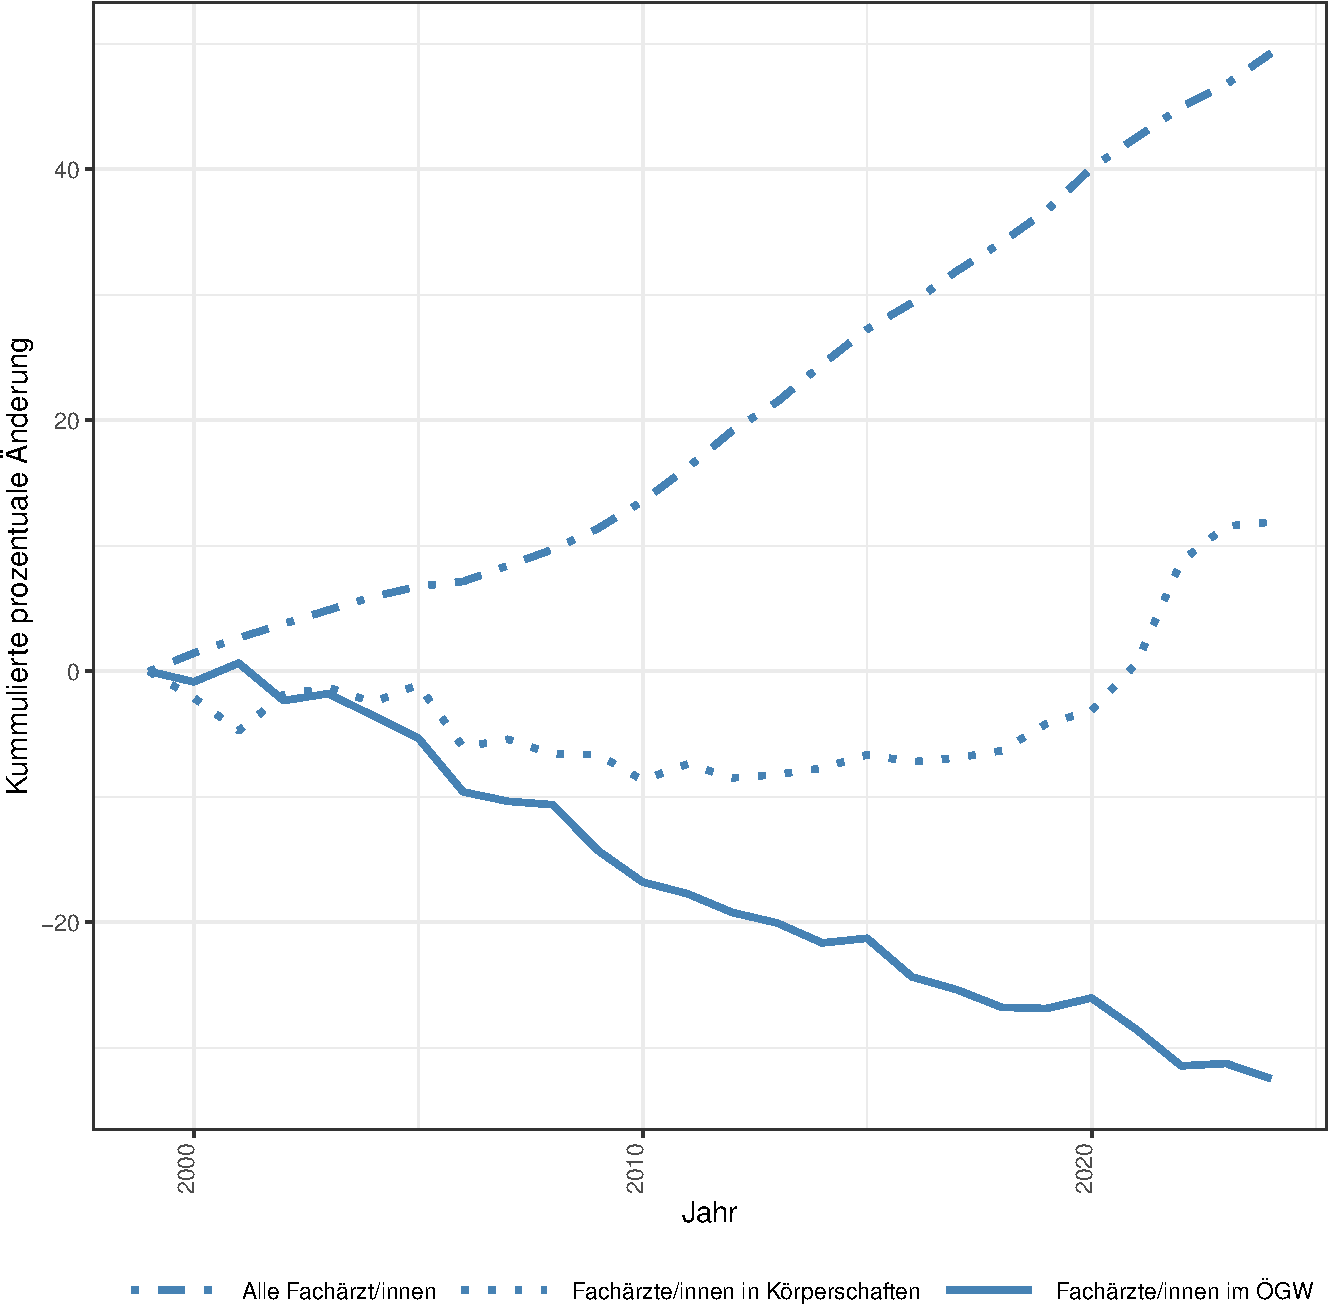
\includegraphics[keepaspectratio]{index_files/figure-pdf/Abbildung 1-1.pdf}}

\textsubscript{Quelle:
\href{https://jakobschumacher.github.io/Update-Facharztmangel-im-oeffentlichen-Gesundheitsdienst/index.qmd.html}{Artikel-Notizbuch}}

\subsubsection{Anteil der Fachärzt/innen
ÖGW}\label{anteil-der-fachuxe4rztinnen-uxf6gw}

\begin{longtable}[]{@{}lr@{}}
\toprule\noalign{}
Tätigkeit & Anzahl im Jahr 2023 \\
\midrule\noalign{}
\endhead
\bottomrule\noalign{}
\endlastfoot
Öffentliches Gesundheitswesen & 724 \\
In Behörden/Körperschaften u. a. & 11700 \\
Gesamt & 428417 \\
\end{longtable}

\textsubscript{Quelle:
\href{https://jakobschumacher.github.io/Update-Facharztmangel-im-oeffentlichen-Gesundheitsdienst/index.qmd.html}{Artikel-Notizbuch}}

\subsection{Nach Region}\label{nach-region}

Bei den Ärztekammern registrierte tätigen Fachärt/innen für Öffentliches
Gesundheitswesen nach Region von 1998 bis 2023 in Deutschland

\subsubsection{Abbildung}\label{abbildung-1}

\pandocbounded{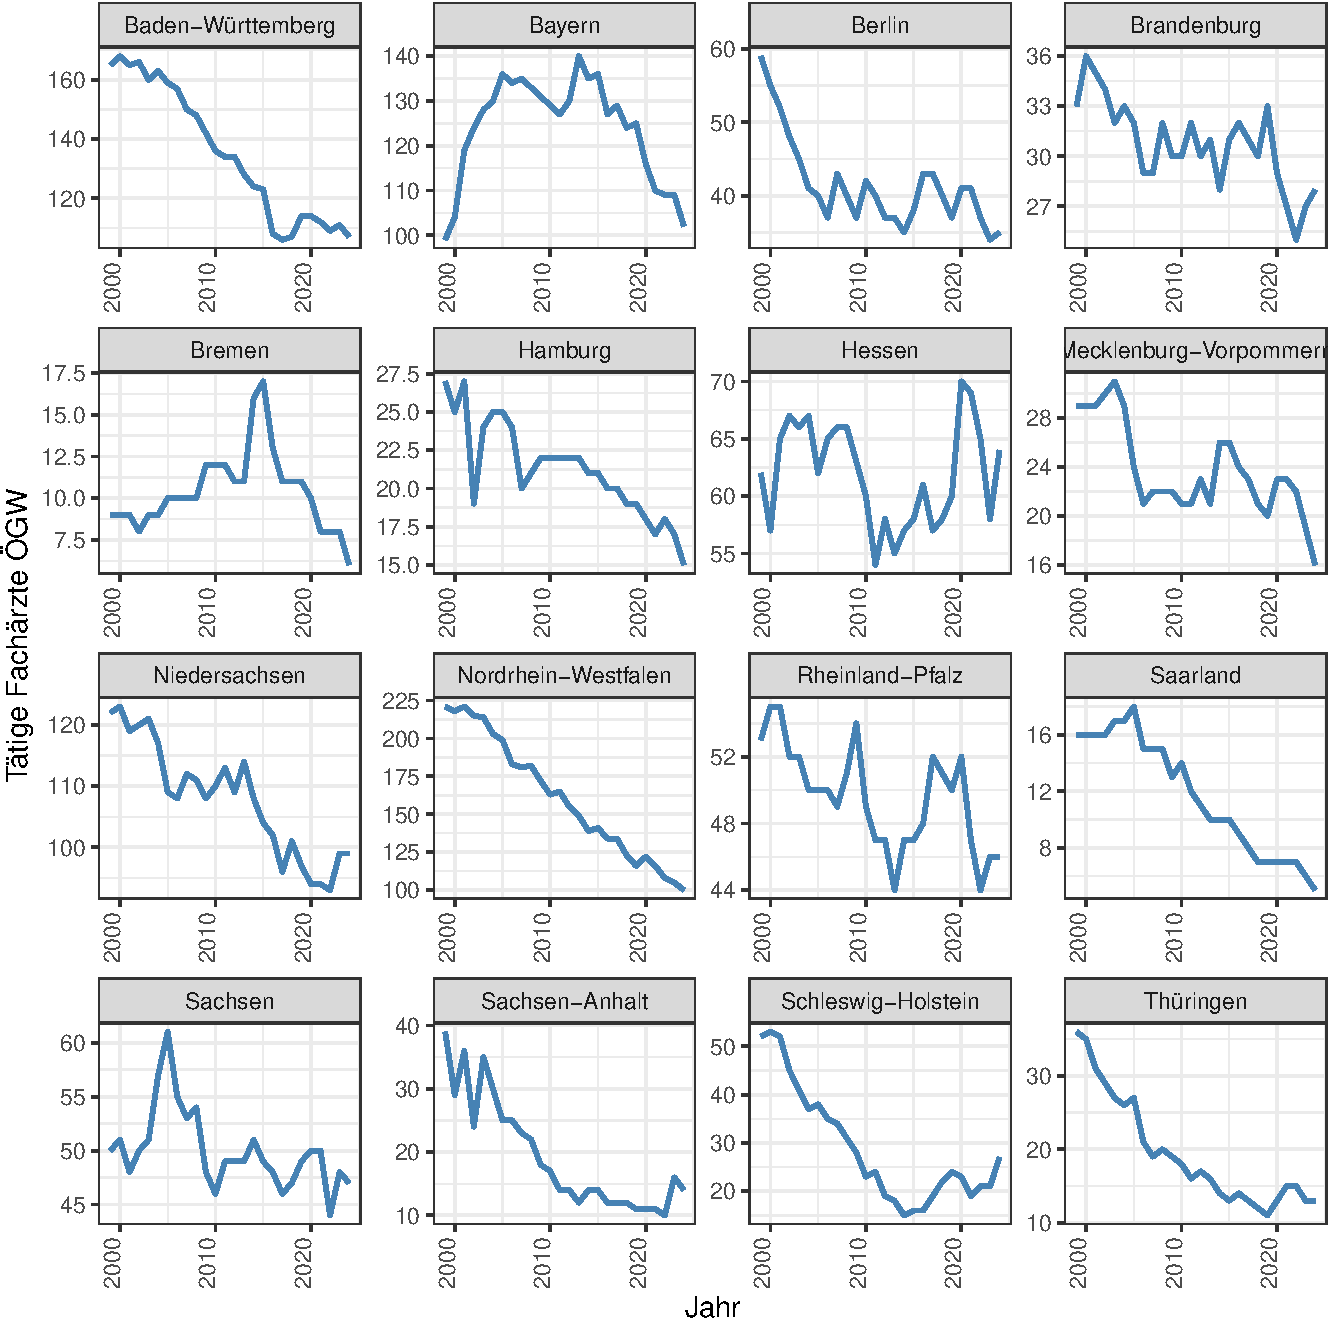
\includegraphics[keepaspectratio]{index_files/figure-pdf/fig2-1.pdf}}

\textsubscript{Quelle:
\href{https://jakobschumacher.github.io/Update-Facharztmangel-im-oeffentlichen-Gesundheitsdienst/index.qmd.html}{Artikel-Notizbuch}}

\subsubsection{Tabelle}\label{tabelle}

\begin{longtable}[]{@{}lrrr@{}}
\toprule\noalign{}
Region & 1998-12-31 & 2023-12-31 & Verlust in Prozent \\
\midrule\noalign{}
\endhead
\bottomrule\noalign{}
\endlastfoot
Saarland & 16 & 5 & -68.8 \\
Sachsen-Anhalt & 39 & 14 & -64.1 \\
Thüringen & 36 & 13 & -63.9 \\
Nordrhein-Westfalen & 221 & 100 & -54.8 \\
Schleswig-Holstein & 52 & 27 & -48.1 \\
Mecklenburg-Vorpommern & 29 & 16 & -44.8 \\
Hamburg & 27 & 15 & -44.4 \\
Berlin & 59 & 35 & -40.7 \\
Baden-Württemberg & 165 & 107 & -35.2 \\
Bremen & 9 & 6 & -33.3 \\
Niedersachsen & 122 & 99 & -18.9 \\
Brandenburg & 33 & 28 & -15.2 \\
Rheinland-Pfalz & 53 & 46 & -13.2 \\
Sachsen & 50 & 47 & -6.0 \\
Bayern & 99 & 102 & 3.0 \\
Hessen & 62 & 64 & 3.2 \\
\end{longtable}

\subsubsection{Tabelle Anzahl pro
100.000}\label{tabelle-anzahl-pro-100.000}

\begin{longtable}[]{@{}lr@{}}
\toprule\noalign{}
Region & Anzahl pro 100.000 (2023) \\
\midrule\noalign{}
\endhead
\bottomrule\noalign{}
\endlastfoot
Saarland & 0.50 \\
Nordrhein-Westfalen & 0.55 \\
Thüringen & 0.61 \\
Sachsen-Anhalt & 0.64 \\
Bayern & 0.76 \\
Hamburg & 0.79 \\
Bremen & 0.87 \\
Schleswig-Holstein & 0.91 \\
Berlin & 0.93 \\
Baden-Württemberg & 0.94 \\
Mecklenburg-Vorpommern & 0.98 \\
Hessen & 1.00 \\
Brandenburg & 1.08 \\
Rheinland-Pfalz & 1.10 \\
Sachsen & 1.15 \\
Niedersachsen & 1.21 \\
\end{longtable}

\subsection{Nach Facharztrichtungen}\label{nach-facharztrichtungen}

Bei den Ärztekammern registrierte tätigen Ärztinnen und Ärzte für
ausgewählte Facharztrichtungen in Deutschland zwischen 1998 und 2017

\subsubsection{Abbildung}\label{abbildung-2}

\pandocbounded{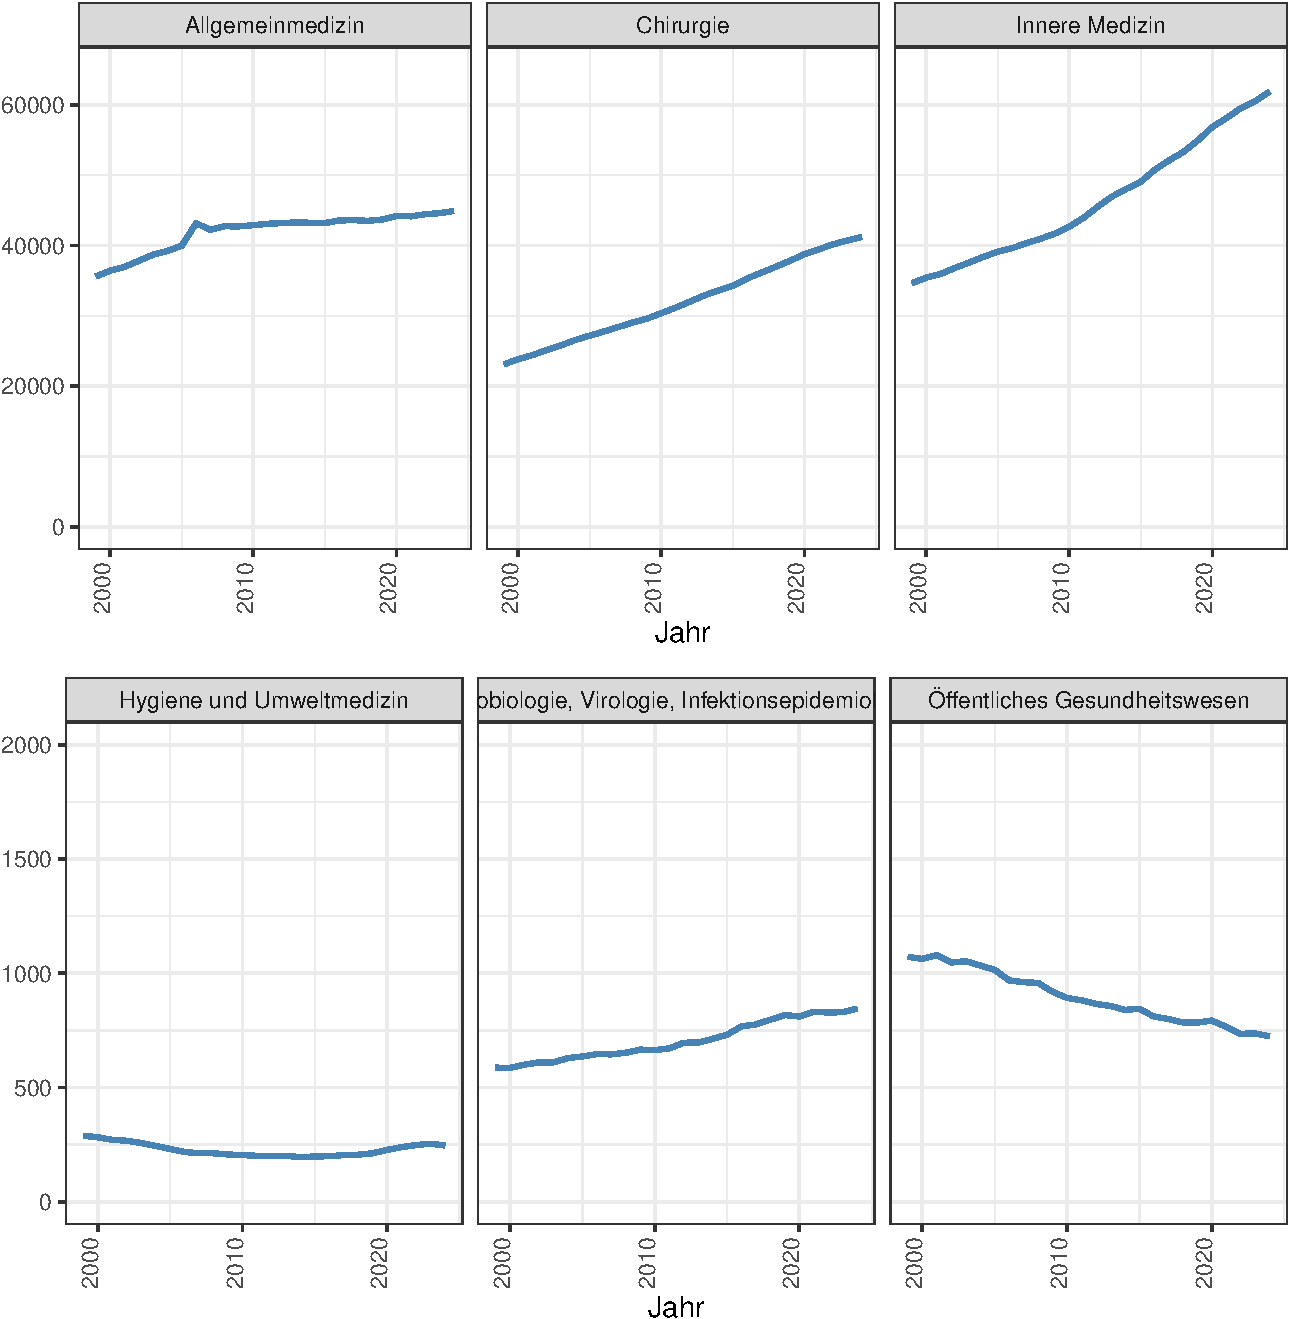
\includegraphics[keepaspectratio]{index_files/figure-pdf/unnamed-chunk-3-1.pdf}}

\textsubscript{Quelle:
\href{https://jakobschumacher.github.io/Update-Facharztmangel-im-oeffentlichen-Gesundheitsdienst/index.qmd.html}{Artikel-Notizbuch}}

\subsubsection{Tabelle}\label{tabelle-1}

\begin{longtable}[]{@{}
  >{\raggedright\arraybackslash}p{(\linewidth - 6\tabcolsep) * \real{0.4098}}
  >{\raggedleft\arraybackslash}p{(\linewidth - 6\tabcolsep) * \real{0.1639}}
  >{\raggedleft\arraybackslash}p{(\linewidth - 6\tabcolsep) * \real{0.1639}}
  >{\raggedleft\arraybackslash}p{(\linewidth - 6\tabcolsep) * \real{0.2623}}@{}}
\toprule\noalign{}
\begin{minipage}[b]{\linewidth}\raggedright
Facharzt
\end{minipage} & \begin{minipage}[b]{\linewidth}\raggedleft
Anzahl im Jahr 1998
\end{minipage} & \begin{minipage}[b]{\linewidth}\raggedleft
Anzahl im Jahr 2023
\end{minipage} & \begin{minipage}[b]{\linewidth}\raggedleft
Kumulierte prozentuale Änderung
\end{minipage} \\
\midrule\noalign{}
\endhead
\bottomrule\noalign{}
\endlastfoot
Biochemie & 93 & 33 & -64.5 \\
Öffentliches Gesundheitswesen & 1072 & 724 & -32.5 \\
Pharmakologie & 492 & 355 & -27.8 \\
Physiologie & 119 & 87 & -26.9 \\
Anatomie & 134 & 101 & -24.6 \\
Hygiene und Umweltmedizin & 289 & 246 & -14.9 \\
Allgemeinmedizin & 35599 & 44912 & 26.2 \\
Hals-Nasen-Ohrenheilkunde & 5172 & 6607 & 27.7 \\
Augenheilkunde & 6305 & 8135 & 29.0 \\
Laboratoriumsmedizin & 924 & 1206 & 30.5 \\
Rechtsmedizin & 220 & 298 & 35.5 \\
Frauenheilkunde und Geburtshilfe & 14327 & 19530 & 36.3 \\
Psychosomatische Medizin und Psychotherapie & 2872 & 4046 & 40.9 \\
Mikrobiologie, Virologie, Infektionsepidemiologie & 587 & 845 & 44.0 \\
Pathologie & 1314 & 1892 & 44.0 \\
Physikalische und Rehabilitative Medizin & 1303 & 1879 & 44.2 \\
Transfusionsmedizin & 381 & 551 & 44.6 \\
Haut- und Geschlechtskrankheiten & 4429 & 6511 & 47.0 \\
Kinder- und Jugendmedizin & 11044 & 16802 & 52.1 \\
Arbeitsmedizin & 2614 & 4101 & 56.9 \\
Urologie & 4186 & 6624 & 58.2 \\
Nuklearmedizin & 724 & 1240 & 71.3 \\
Radiologie & 5725 & 9938 & 73.6 \\
Chirurgie & 23113 & 41233 & 78.4 \\
Innere Medizin & 34653 & 61899 & 78.6 \\
Mund-Kiefer-Gesichtschirurgie & 1048 & 1903 & 81.6 \\
Anästhesiologie & 13779 & 27572 & 100.1 \\
Humangenetik & 151 & 410 & 171.5 \\
Neurochirurgie & 867 & 2713 & 212.9 \\
Kinder- und Jugendpsychiatrie und -psychotherapie & 910 & 2855 &
213.7 \\
Psychiatrie und Psychotherapie & 3760 & 12957 & 244.6 \\
Strahlentherapie & 457 & 1609 & 252.1 \\
Neurologie & 1961 & 9636 & 391.4 \\
\end{longtable}

\textsubscript{Quelle:
\href{https://jakobschumacher.github.io/Update-Facharztmangel-im-oeffentlichen-Gesundheitsdienst/index.qmd.html}{Artikel-Notizbuch}}

\subsection{Nach Alter}\label{nach-alter}

Bei den Ärztekammern registrierte tätige Ärztinnen und Ärzte mit der
Facharztbezeichnung Öffentliches Gesundheitswesen nach Alter in
Deutschland von 1998 bis 2023

\subsubsection{Abbildung über Zeit}\label{abbildung-uxfcber-zeit}

\pandocbounded{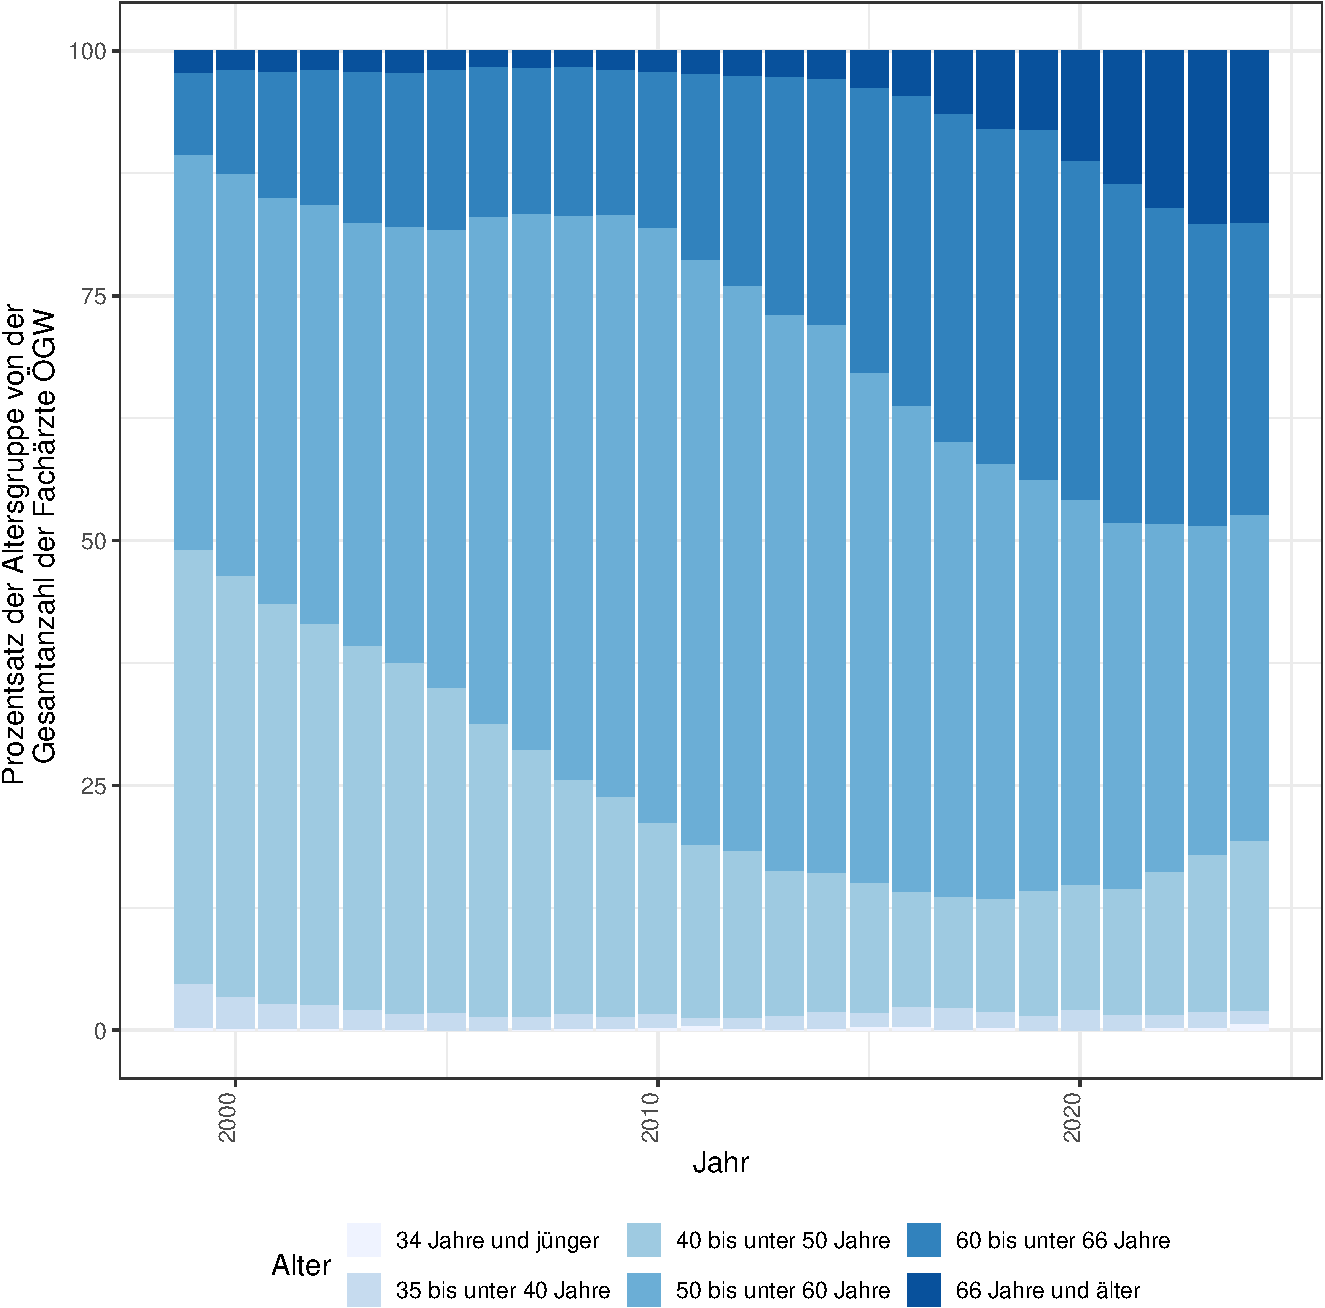
\includegraphics[keepaspectratio]{index_files/figure-pdf/Abbildung 4-1.pdf}}

\textsubscript{Quelle:
\href{https://jakobschumacher.github.io/Update-Facharztmangel-im-oeffentlichen-Gesundheitsdienst/index.qmd.html}{Artikel-Notizbuch}}

\subsubsection{Abbildung
Jahresvergleich}\label{abbildung-jahresvergleich}

\pandocbounded{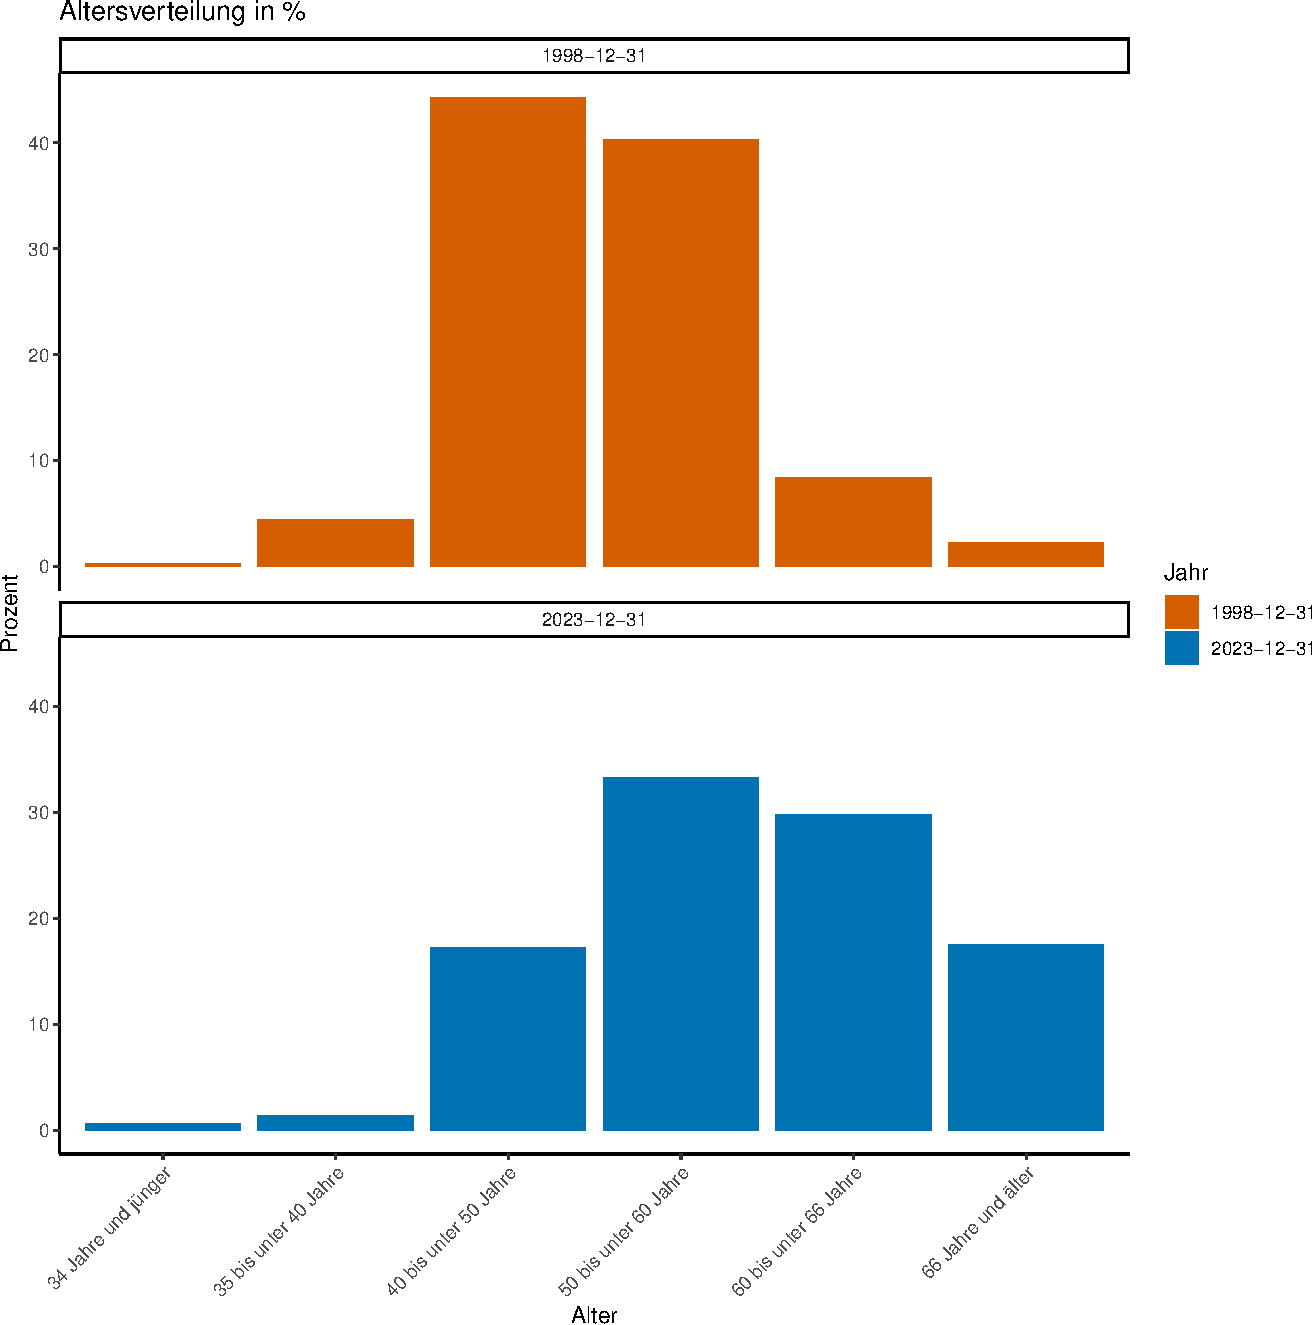
\includegraphics[keepaspectratio]{index_files/figure-pdf/unnamed-chunk-5-1.pdf}}

\textsubscript{Quelle:
\href{https://jakobschumacher.github.io/Update-Facharztmangel-im-oeffentlichen-Gesundheitsdienst/index.qmd.html}{Artikel-Notizbuch}}

\subsubsection{Tabelle}\label{tabelle-2}

\begin{longtable}[]{@{}llrrr@{}}
\toprule\noalign{}
Jahr & Alter & n & total\_per\_year & percent \\
\midrule\noalign{}
\endhead
\bottomrule\noalign{}
\endlastfoot
1998-12-31 & 34 Jahre und jünger & 3 & 1072 & 0.28 \\
1998-12-31 & 35 bis unter 40 Jahre & 48 & 1072 & 4.48 \\
1998-12-31 & 40 bis unter 50 Jahre & 475 & 1072 & 44.31 \\
1998-12-31 & 50 bis unter 60 Jahre & 432 & 1072 & 40.30 \\
1998-12-31 & 60 bis unter 66 Jahre & 90 & 1072 & 8.40 \\
1998-12-31 & 66 Jahre und älter & 24 & 1072 & 2.24 \\
2023-12-31 & 34 Jahre und jünger & 5 & 724 & 0.69 \\
2023-12-31 & 35 bis unter 40 Jahre & 10 & 724 & 1.38 \\
2023-12-31 & 40 bis unter 50 Jahre & 125 & 724 & 17.27 \\
2023-12-31 & 50 bis unter 60 Jahre & 241 & 724 & 33.29 \\
2023-12-31 & 60 bis unter 66 Jahre & 216 & 724 & 29.83 \\
2023-12-31 & 66 Jahre und älter & 127 & 724 & 17.54 \\
\end{longtable}

\textsubscript{Quelle:
\href{https://jakobschumacher.github.io/Update-Facharztmangel-im-oeffentlichen-Gesundheitsdienst/index.qmd.html}{Artikel-Notizbuch}}

\subsection{Nach Geschlecht}\label{nach-geschlecht}

\subsubsection{Abbildung}\label{abbildung-3}

\pandocbounded{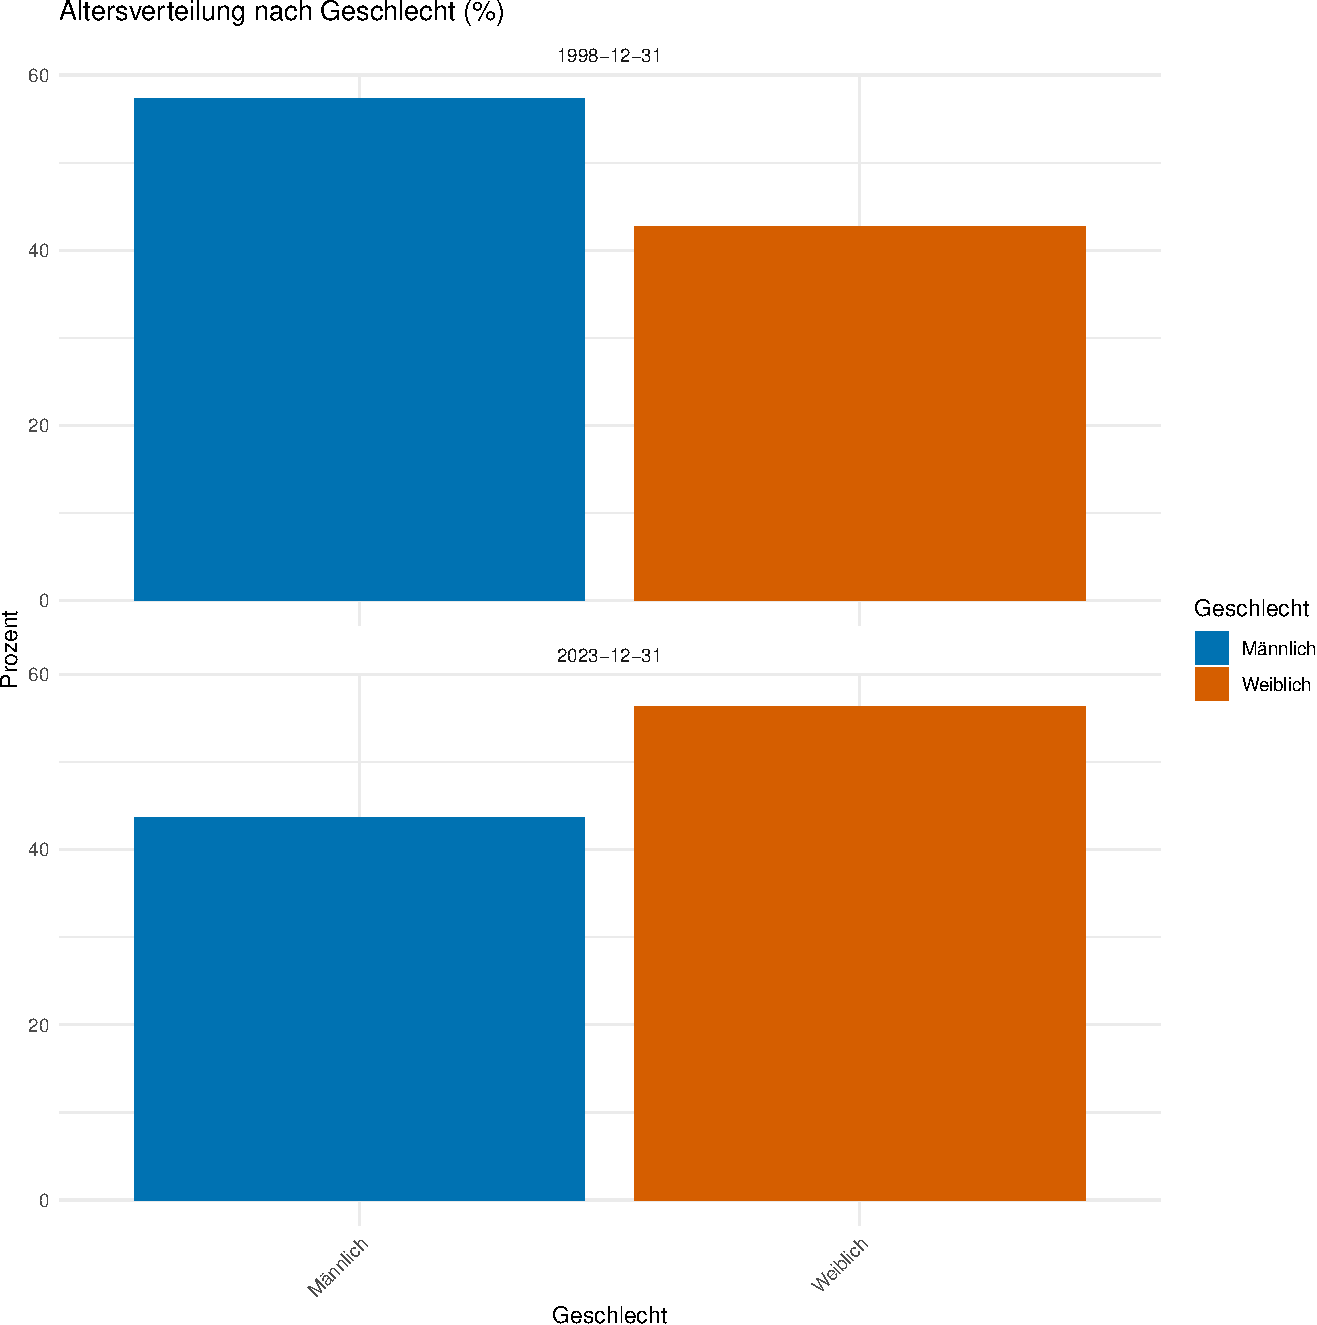
\includegraphics[keepaspectratio]{index_files/figure-pdf/unnamed-chunk-7-1.pdf}}

\textsubscript{Quelle:
\href{https://jakobschumacher.github.io/Update-Facharztmangel-im-oeffentlichen-Gesundheitsdienst/index.qmd.html}{Artikel-Notizbuch}}

\subsubsection{Tabelle}\label{tabelle-3}

\begin{longtable}[]{@{}llrr@{}}
\toprule\noalign{}
Jahr & Geschlecht & n & percent \\
\midrule\noalign{}
\endhead
\bottomrule\noalign{}
\endlastfoot
1998-12-31 & Männlich & 614 & 57.28 \\
1998-12-31 & Weiblich & 458 & 42.72 \\
2023-12-31 & Männlich & 316 & 43.65 \\
2023-12-31 & Weiblich & 408 & 56.35 \\
\end{longtable}

\textsubscript{Quelle:
\href{https://jakobschumacher.github.io/Update-Facharztmangel-im-oeffentlichen-Gesundheitsdienst/index.qmd.html}{Artikel-Notizbuch}}

\subsection{Alterspyramide}\label{alterspyramide}

Bei den Ärztekammern registrierte tätige Ärztinnen und Ärzte mit der
Facharztbezeichnung ÖGW nach Geschlecht und Alter (Alterspyramide) in
Deutschland von 1998 bis 2023

\pandocbounded{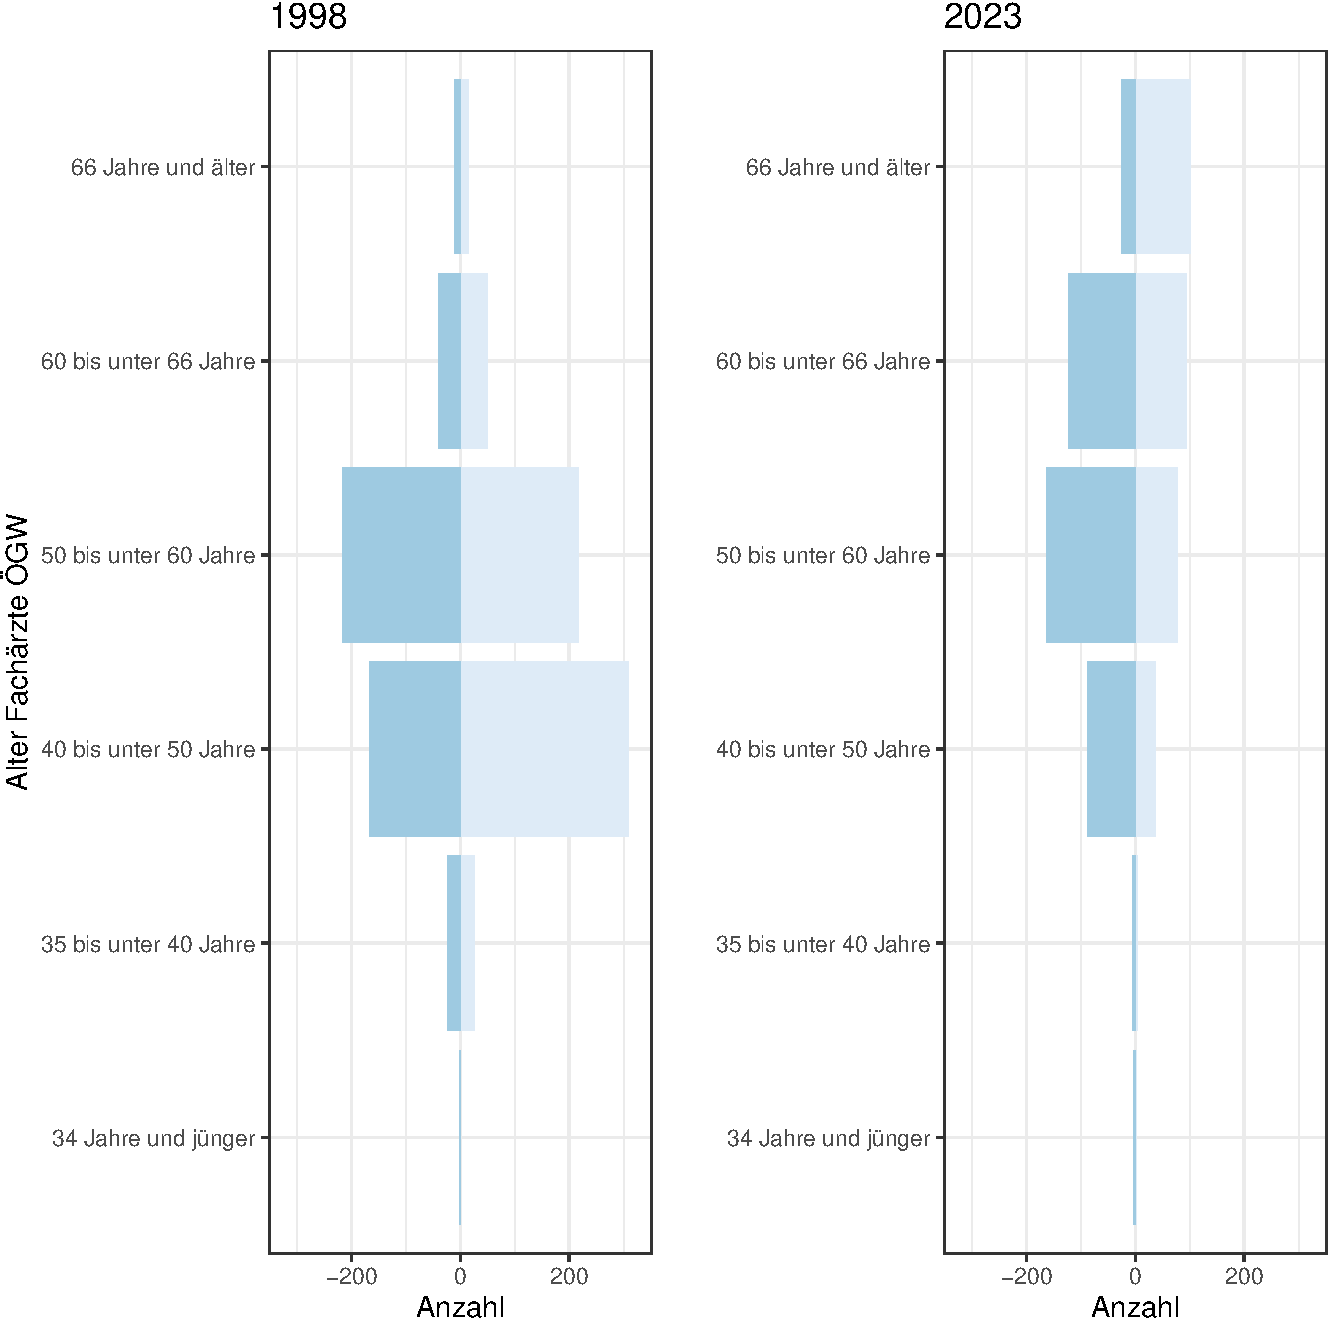
\includegraphics[keepaspectratio]{index_files/figure-pdf/Abbildung 5-1.pdf}}

\textsubscript{Quelle:
\href{https://jakobschumacher.github.io/Update-Facharztmangel-im-oeffentlichen-Gesundheitsdienst/index.qmd.html}{Artikel-Notizbuch}}

\section{Diskussion}\label{diskussion}

Die Ergebnisse unserer Untersuchung zeigen, dass die COVID-19-Pandemie
den rückläufigen Trend bei der Anzahl der Fachärzte für Öffentliches
Gesundheitswesen nicht aufhalten konnte. Trotz der erheblichen
Aufmerksamkeit, die der Öffentliche Gesundheitsdienst während der
Pandemie erhielt, und der damit einhergehenden gestiegenen
gesellschaftlichen Anerkennung seiner Bedeutung, setzte sich der bereits
von Tinnemann et al.~(2021) dokumentierte Abwärtstrend fort. Dies ist
besonders bemerkenswert, da die Pandemie die zentrale Rolle des ÖGD im
Gesundheitssystem deutlich hervorgehoben hat.

Paradoxerweise berichten die Bundesländer gleichzeitig von einem Anstieg
der Gesamtbeschäftigtenzahl in den lokalen Gesundheitsämtern. Diese
Diskrepanz lässt sich vermutlich teilweise durch die Art der neu
geschaffenen Stellen erklären. Im Rahmen des ``Pakts für den
Öffentlichen Gesundheitsdienst'' wurden bis Ende 2022 bundesweit etwa
XXXX Vollzeitäquivalente geschaffen. Vermutlich wurden diese Stellen
überwiegend mit nicht-ärztlichem Personal besetzt, darunter
Verwaltungskräfte, Hygienekontrolleure und Sozialarbeiter. Die Fachärzte
für ÖGW konnte von dieser personellen Aufstockung bislang offenbar nicht
profitieren.

Diese Entwicklung ist bedenklich, da gerade die fachärztliche Expertise
für die Wahrnehmung hoheitlicher Aufgaben und die adäquate Versorgung
vulnerabler Bevölkerungsgruppen unverzichtbar ist. Die anhaltende
Überalterung der Fachärzteschaft für ÖGW, die bereits vor der Pandemie
mit einem Anstieg des Anteils der über 50-Jährigen auf XXX dokumentiert
wurde, verschärft diese Problematik zusätzlich und deutet auf einen
drohenden weiteren Rückgang in den kommenden Jahren durch
Pensionierungen hin.

Bei der Interpretation unserer Ergebnisse müssen einige Limitationen
berücksichtigt werden. Insbesondere könnte der Zeitpunkt unserer
Erhebung zu früh nach der akuten Pandemiephase liegen, um mögliche
positive Effekte auf die Nachwuchsgewinnung vollständig abzubilden. Die
Ausbildung zum Facharzt für Öffentliches Gesundheitswesen erfordert nach
dem Medizinstudium eine mehrjährige Weiterbildung. Daher könnten sich
eventuelle pandemiebeeinflusste Karriereentscheidungen junger Ärztinnen
und Ärzte erst mit zeitlicher Verzögerung in den Statistiken
niederschlagen. Eine Folgeerhebung in drei bis fünf Jahren könnte
feststellen, ob die während der Pandemie gestiegene Aufmerksamkeit für
Public Health langfristig zu einem verstärkten Interesse an der
Facharztweiterbildung ÖGW geführt hat.

Die anhaltend geringe Anzahl an Fachärzten für ÖGW steht im Widerspruch
zu den steigenden Anforderungen an den ÖGD und den Lehren aus der
Pandemie. Während der ``Pakt für den Öffentlichen Gesundheitsdienst''
wichtige Verbesserungen eingeleitet hat, scheint die spezifische
Förderung des fachärztlichen Nachwuchses bislang nicht ausreichend
berücksichtigt worden zu sein. Die von der Studie aufgezeigte Diskrepanz
zwischen allgemeiner Personalaufstockung und dem anhaltenden Mangel an
Fachärzten für ÖGW unterstreicht die Notwendigkeit gezielter Maßnahmen
zur Attraktivitätssteigerung dieser Fachdisziplin.




\end{document}
